%%%%%%%%%%%%%%%%%%%%%%%%%%%%%%%%%%%%%%%%%

% Simple Sectioned Essay Template
% LaTeX Template
%
% This template has been downloaded from:
% http://www.latextemplates.com
%
% Note:
% The \lipsum[#] commands throughout this template generate dummy text
% to fill the template out. These commands should all be removed when 
% writing essay content.
%
%%%%%%%%%%%%%%%%%%%%%%%%%%%%%%%%%%%%%%%%%

%----------------------------------------------------------------------------------------
%	PACKAGES AND OTHER DOCUMENT CONFIGURATIONS
%----------------------------------------------------------------------------------------

\documentclass[12pt]{article} % Default font size is 12pt, it can be changed here

\usepackage{geometry} % Required to change the page size to A4
\usepackage{subfigure}
\usepackage{placeins}
\usepackage{placeins}
\usepackage{hyperref}
\geometry{a4paper} % Set the page size to be A4 as opposed to the default US Letter

\usepackage{graphicx} % Required for including pictures

\usepackage{float} % Allows putting an [H] in \begin{figure} to specify the exact location of the figure
\usepackage{amssymb} % Allows putting an [H] in \begin{figure} to specify the exact location of the figure
\usepackage{wrapfig} % Allows in-line images such as the example fish picture

\usepackage{lipsum} % Used for inserting dummy 'Lorem ipsum' text into the template

\linespread{1.2} % Line spacing

%\setlength\parindent{0pt} % Uncomment to remove all indentation from paragraphs

\graphicspath{{./Pictures/}} % Specifies the directory where pictures are stored

\begin{document}
\title{Netwerken en systeembeveiliging\\ Assignment 1}
\author{Inge Becht}
\date{\today}

\maketitle
 \begin{enumerate}
     \item IP-address of ss64.com : 216.92.29.160\\
           IP-address of the sending computer : 145.18.214.201\\
    \item 8 HTTP GET messages were sent.
        I used filter \texttt{http and ip.src == 145.18.214.201 and ip.dst ==
        216.92.29.160}\
    \item 
        I chose the \texttt{GET /bash.ping.html HTTP/1.1} message. The included
        protocols were:
        \begin{itemize}
            \item Internet Protocol version 4 (IPv4)
            \item Transmission Control Protocol
            \item Hypertext Transfer Protocol (HTTP)
        \end{itemize}
    \item If by your computer is meant the computer from which the dump is taken: 
        8 HTTP OK messages from ss64.com(filter : \texttt{http and ip.src ==
        145.18.214.201 and ip.dst == 216.92.29.160} )
    \item{ By filtering on \texttt{http} the first two messages are a HTTP GET and
            HTTP OK messages. Then, choosing the \texttt{Seconds since Previously
            Displayed Packet} option as the time display you get approximately
            0.4345 seconds.
         }
    \item Yes, 6 images were sent:
        \begin{itemize}
            \item ss64.gif
            \item bash-l.gif
            \item syntax-r.gif
            \item top-4.gif
            \item roll-left.png
            \item roll-right.png
        \end{itemize}
    \item Done by right clicking on the packet and choosing \texttt{print}. (You
        do have to make certain that the things you want to print are opened in
        the list of information when you double click on a packet).
        The packets from which the messages were extracted are \texttt{GET
        /bash/ping.html HTTP/1.1} (entry 86) and  \texttt{HTTP/1.1 200 OK
        (text/html)} (entry 114). The messages can be seen in Appendix A(at the
        back).
    \item 
        Computer sent 38 packets(total of 5650 bytes) to the server and
        ss64.com sent
        39 packets(total of 32908 bytes) to the computer
        There is a lot more received by the computer than sent, this because all the images needed to
        be sent to the computer and the computer only asked for permission to
        get this content. So the received data contains more bytes than the
        data sent out.
   \item
    \begin{figure}[l!]
        \centering
        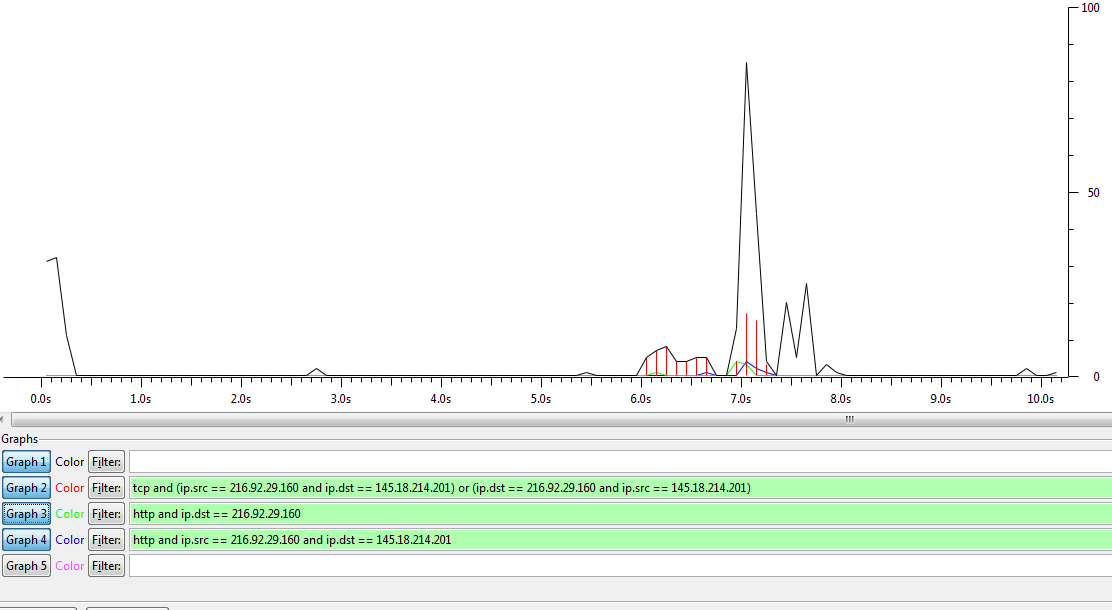
\includegraphics[width=1.2\textwidth]{data.png}
        \caption{Packet distribution}
        \label{ref:simple}
    \end{figure}

    See figure \ref{ref:simple} for the graph. This graph seems not all that
    clear to me so also see figure \ref{ref:simple2} for the HTTP messages sent between
    ss64.com and the computer. Here the seems to be consistent with
    earlier answers( 8 HTTP GET messages were sent and 8 received)


\begin{figure}[l!]
    \centering
    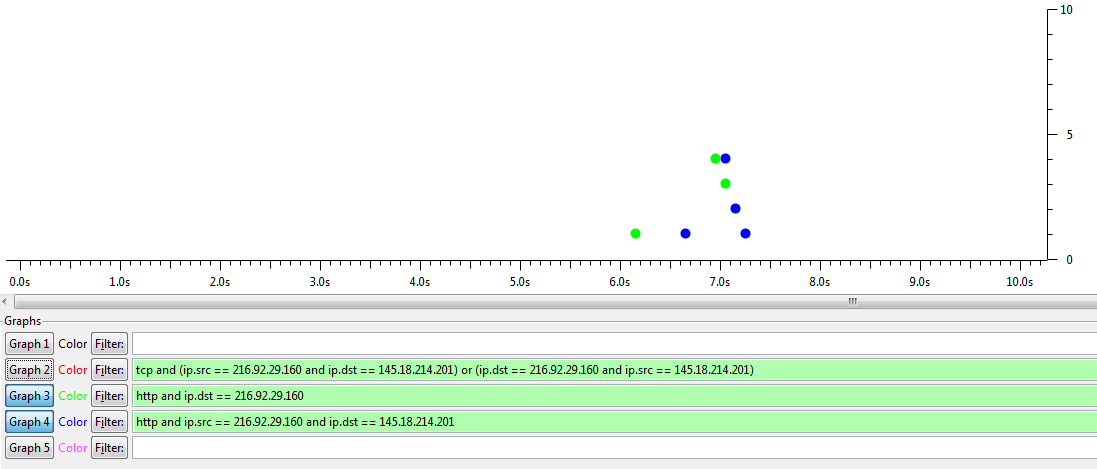
\includegraphics[width=1.2\textwidth]{data2.png}
    \caption{HTTP GET and OK distribution between computer and ss64.com}
    \label{ref:simple2}
\end{figure}
\FloatBarrier
    \item The passwords sent are \texttt{wrong!} and \texttt{network}.
        First I filtered on \texttt{http} to show all readable data. Here I found
        the ip 145.100.102.253 making a HTTP GET request towards ip
        145.00.102.153. So the first ip belonged to the computer and the other
        ip to some site that the computer tried to connect to. In the HTML sent to the
        computer I could read when the user did not have access to the page
        tried to visit and when he did (entry 13 and 25 respectively). So then I
        read the data in the requests, and found the authorization section with the
        credentials and the things that were different between both requests.
        The correct password is network. This because after applying this
        password the computer receives the sites content that shows it was the
        right password. I myself went to
        the protected page as well, to check if this
        password worked (together with the username wireshark-student) and it
        worked.

 \end{enumerate}
\clearpage
% appendix
 \appendix
 \section{Data for question 7}
 \label{app}
  Data from \texttt{GET
        /bash/ping.html HTTP/1.1} (entry 86):\\
        \begin{verbatim}
No. Time         Source          Destination    Protocol Length Info
86  6.195787000  145.18.214.201  216.92.29.160  HTTP     485    GET /bash/ping.html HTTP/1.1 

Frame 86: 485 bytes on wire (3880 bits), 
                            485 bytes captured (3880 bits) on interface 0
Ethernet II, Src: Apple_11:f3:14 (e4:ce:8f:11:f3:14), 
                            Dst: Cisco_45:2c:00 (00:0a:42:45:2c:00)
Internet Protocol Version 4, Src: 145.18.214.201 (145.18.214.201), 
                            Dst: 216.92.29.160 (216.92.29.160)
Transmission Control Protocol, Src Port: 50839 (50839), 
                            Dst Port: http (80), Seq: 1, Ack: 1, Len: 419
Hypertext Transfer Protocol
    GET /bash/ping.html HTTP/1.1\r\n
    Host: ss64.com\r\n
    Connection: keep-alive\r\n
    Cache-Control: max-age=0\r\n
    User-Agent: Mozilla/5.0 (Macintosh; Intel Mac OS X 10_7_5) 
                        AppleWebKit/537.4 (KHTML, like Gecko) Chrome/22.0.1229.94 Safari/537.4\r\n
    Accept: text/html,application/xhtml+xml,application/xml;q=0.9,*/*;q=0.8\r\n
    Accept-Encoding: gzip,deflate,sdch\r\n
    Accept-Language: en-US,en;q=0.8\r\n
    Accept-Charset: ISO-8859-1,utf-8;q=0.7,*;q=0.3\r\n
    \r\n
    [Full request URI: http://ss64.com/bash/ping.html]
    \end{verbatim}
    Data from  \texttt{HTTP/1.1 200 OK
    (text/html)} (entry 114):\\
    \begin{verbatim}

    No.     Time           Source                Destination           Protocol Length Info
    114 6.630232000    216.92.29.160         145.18.214.201        HTTP     1341   HTTP/1.1 200 OK  (text/html)

Frame 114: 1341 bytes on wire (10728 bits), 1341 bytes captured (10728 bits) on interface 0
Ethernet II, Src: Cisco_45:2c:00 (00:0a:42:45:2c:00), Dst: Apple_11:f3:14 (e4:ce:8f:11:f3:14)
Internet Protocol Version 4, Src: 216.92.29.160 (216.92.29.160), Dst: 145.18.214.201 (145.18.214.201)
Transmission Control Protocol, Src Port: http (80), Dst Port: 50839 (50839), Seq: 11088, Ack: 420, Len: 1275
[10 Reassembled TCP Segments (12362 bytes): #96(279), #101(1351), #102(1351), #103(1351), #106(1351), #107(1351), #109(1351), #111(1351), #112(1351), #114(1275)]
Hypertext Transfer Protocol
    HTTP/1.1 200 OK\r\n
    Date: Tue, 23 Oct 2012 14:21:03 GMT\r\n
    Server: Apache/2.2.22\r\n
    Last-Modified: Mon, 27 Aug 2012 10:50:53 GMT\r\n
    ETag: "2f33-4c83d197c9d40"\r\n
    Accept-Ranges: bytes\r\n
    Content-Length: 12083\r\n
    Keep-Alive: timeout=5, max=100\r\n
    Connection: Keep-Alive\r\n
    Content-Type: text/html\r\n
    \r\n
Line-based text data: text/html
    <!DOCTYPE HTML PUBLIC "-//W3C//DTD HTML 4.01 Transitional//EN" "http://www.w3.org/TR/html4/loose.dtd"><html>\n
    <head>\n
    <link rel="STYLESHEET" href="../main.css" type="text/css">\n
    <title>ping Man Page | SS64.com</title>\n
    <meta http-equiv="Content-Type" content="text/html; charset=utf-8">\n
    </head><!-- #BeginLibraryItem "/Library/head_bash.lbi" --><div id="nav-menu"><ul>\n
    <li><a class="rl" href="../index.html"><img src="../images/ss64.gif" alt="Home" width="115" height="47" title="Home"></a></li>\n
    <li><a class="rl" href="../bash"><img src="../images/bash-l.gif" alt="bash" width="115" height="47" title="bash"></a></li>\n
    <li><form action="http://www.google.com/search" method="get" style="margin:0px;padding:0px;">\n
    <input name="q" type="text" alt="search" id="question" size="20" maxlength="255">\n
    <input class="submit" type="submit" value="Search" id="btn">\n
    <input type="hidden" name="sitesearch" value="ss64.com/bash/">\n
    </form></li>\n
    <li><a class="rr" href="syntax.html"><img src="../images/syntax-r.gif" width="115" height="47" title="Bash Syntax"></a></li></ul>\n
    </div> <!-- #EndLibraryItem --><h1>ping</h1> \n
    <p>Test a network connection. When using ping for fault isolation, it should first be run on the local host, to verify that the local network interface is up and running.\n
    Then, hosts and gateways further and further away should be `pinged'.</p>\n
    <pre>Syntax<br>      ping [<i>options</i>] <i>destination_host</i>\n
    \n
    Options\n
    \n
       -a         Audible ping. \n
    \n
       -A         Adaptive ping. Interpacket interval adapts to round-trip time, \n
                  so that effectively not more than one (or more, if preload is set) unanswered probes\n
                  present in the network. Minimal interval is 200msec for not super-user.\n
                  On networks with low rtt this mode is essentially equivalent to flood mode. \n
    \n
       -b         Allow pinging a broadcast address. \n
    \n
       -B         Do not allow ping to change source address of probes. The address is bound to one selected when ping starts.\n
    \n
       -c <i>count</i>   Stop after sending (and receiving) <i>count</i> ECHO_RESPONSE packets.\n
    \n
       -d         Debug, Set the SO_DEBUG option on the socket being used.\n
    \n
       -F <i>flow_label</i>  Allocate and set 20 bit flow label on echo request packets. (Only ping6).\n
                      If value is zero, kernel allocates random flow label.\n
    \n
       -f         Flood ping, output packets as fast as they come back or 100 times per second.\n
    \n
       -i <i>wait</i>    Set an interval of <i>wait </i>seconds between sending each packet. default=one second.\n
                  Only super-user may set <i>wait</i> to values less 0.2 seconds.\n
                  (incompatible with -f)\n
    \n
       -I <i>interface address<br></i>              Set source address to specified <i>interface_address</i>.\n
                  Argument may be numeric IP address or name of device.\n
                  Required when pinging an IPv6 link-local address.\n
    \n
       -l <i>preload</i> If preload is specified, ping sends that many packets as fast as\n
                  possible before falling into its normal mode of behavior.\n
                  Only the super-user may select preload more than 3.\n
    \n
       -L         Suppress loopback of multicast packets.\n
                  only applies if the ping destination is a multicast address.\n
    \n
       -n         Numeric output only. No attempt will be made to lookup symbolic\n
                  names for host addresses.\n
       -p <i>pattern</i>\n
                  Specify up to 16 `pad' bytes to fill out the packet sent.\n
                  This is useful for diagnosing data-dependent problems in a\n
                  network. eg, `-p ff' will fill the packet sent with all ones.\n
    \n
       -q         Quiet output. Only display the summary lines at startup time and when finished.\n
     \n
       -Q <i>tos    </i> Set Quality of Service -related bits in ICMP datagrams. <i>tos</i> can be a decimal or hex number.\n
                  Multiple TOS bits should not be set simultaneously. For detail see RFC1349 and RFC2474\n
    \n
       -R         Record route(IPv4 only). Includes the RECORD_ROUTE option in the ECHO_REQUEST packet and\n
                  display the route buffer on returned packets.\n
                  Note that the IP header is only large enough for nine such routes.\n
                  Many hosts ignore or discard this option.\n
     \n
       -r         Bypass the normal routing tables and send directly to a host on an attached network.\n
                  If the host is not on a directly-attached network, an error is returned.\n
                  This option can be used to ping a local host through an interface that has no route through it\n
                  (e.g., after the interface was dropped by routed(8)).\n
    \n
       -s <i>packetsize\n
                </i>  The number of data bytes to be sent. The default is 56, which translates into\n
                  64 ICMP data bytes when combined with the 8 bytes of ICMP header data.\n
    \n
       -S <i>sndbuf</i>  Set socket <i>sndbuf</i>. If not specified, it is selected to buffer not more than one packet. <br>\n
       -t <i>ttl</i>     Set the IP Time to Live. <br>\n
       -T <i>timestamp_option</i><br>              Set special IP timestamp options, either 'tsonly' (only timestamps),\n
                  'tsandaddr' (timestamps and addresses)\n
                  or 'tsprespec host1 [host2 [host3 [host4]]]' (timestamp prespecified hops). <br>\n
       -M <i>hint</i>    Select Path MTU Discovery strategy. <i>hint</i> may be either 'do' (prohibit fragmentation,\n
                  even local one), 'want' (do PMTU discovery, fragment locally when packet size is large),\n
                  or 'dont' (do not set DF flag). <br>\n
       -U         Print full user-to-user latency (the old behaviour).\n
                  Normally ping prints network round trip time, which can be different f.e. due to DNS failures.\n
    \n
       -v         Verbose output. ICMP packets other than ECHO_RESPONSE that are received are listed.\n
     \n
    </pre>\n
    <p>\n
    Ping is intended for use in network testing, measurement and management. Because of the load it can impose on the network, it is unwise to use ping during normal operations or from automated scripts. </p>\n
    [truncated] <p>If ping does not receive any reply packets at all it will exit with code 1. If a packet <i>count</i> and <i>deadline</i> are both specified, and fewer than <i>count</i> packets are received by the time the <i>deadline</i> ha
    <p>PING is <a href="http://ftp.arl.mil/~mike/ping.html">named</a> after the sound that a sonar makes.</p>\n
    [truncated] <p>Ping response times below 10 milliseconds often have low accuracy. A time of 10 milliseconds is roughly equal to a distance of 1860 Miles, travelling a straight line route  at the speed of light, (or a round trip of 2 \303\2
    <p><b>Flood Ping</b><br>\n
    [truncated] For every ECHO_REQUEST sent a period `.' is printed, while for every ECHO_REPLY received a backspace is printed. This provides a rapid display of how many packets are being dropped. Only the super-user may use this option. This
    [truncated] <p>Round-trip times and packet loss statistics are computed. If duplicate packets are received, they are not included in the packet loss calculation, although the round trip time of these packets is used in calculating the mini
    <p>Flood pinging is not recommended in general, and flood pinging the broadcast address should only be done under very controlled conditions.</p>\n
    <p><b>ICMP Packet Details</b><br>\n
    [truncated] An IP header without options is 20 bytes. An ICMP ECHO_REQUEST packet contains an additional 8 bytes worth of ICMP header followed by an arbitrary amount of data. When a packetsize is given, this indicated the size of this extr
    [truncated] <p> If the data space is at least eight bytes large, ping uses the first eight bytes of this space to include a timestamp which it uses in the computation of round trip times. If less than eight bytes of pad are specified, no r
    <p><b>Duplicate and Damaged Packets</b><br>\n
    Ping will report duplicate and damaged packets. <br>\n
    Duplicate packets are rarely; if ever; a good sign, although the presence of low levels of duplicates may not always be cause for alarm.<br>\n
    Damaged packets are a serious cause for alarm and often indicate broken hardware somewhere in the ping packet's path (in the network or in the hosts).</p>\n
    <p><b>Different Data Patterns</b><br>\n
    The (inter)network layer should never treat packets differently depending on the data contained in the data portion. Unfortunately, data-dependent<br>\n
    [truncated] problems have been known to sneak into networks and remain undetected for long periods of time. If you have a data-dependent problem you will probably have to do a lot of testing to find it. If you are lucky, you may manage to 
    <p><b>TTL Details</b><br>\n
    [truncated] The <a href="http://en.wikipedia.org/wiki/Time_to_live">Time To Live</a>, (TTL) value of an IP packet represents the maximum number of IP routers that the packet can go through before being thrown away. In current practice you 
    <p> The TCP/IP specification states that the TTL field for TCP packets should be set to 60, but many systems use smaller values (4.3 BSD uses 30, 4.2 used 15).</p>\n
    [truncated] <p> The maximum possible value of this field is 255, and most Unix systems set the TTL field of ICMP ECHO_REQUEST packets to 255. This is why you will find you can `ping' some hosts, but not reach them with telnet(1) or <a href
    <p> In normal operation ping prints the ttl value from the packet it receives. When a remote system receives a ping packet, it can do one of three things with the TTL field in its response:</p>\n
    <ul>\n
    <li> Not change it; this is what Berkeley Unix systems did before the 4.3BSD-Tahoe release. In this case the TTL value in the received packet will be 255 minus the number of routers in the round-trip path.</li>\n
    <li> Set it to 255; this is what current Berkeley Unix systems do. In this case the TTL value in the received packet will be 255 minus the number of routers in the path from the remote system to the pinging host.</li>\n
    <li> Set it to some other value. Some machines use the same value for ICMP packets that they use for TCP packets, for example either 30 or 60. Others may use completely wild values.</li>\n
    </ul>\n
    <p class="quote"><i>&ldquo;There's a Nong Nang Ning, Where the trees go Ping!&rdquo; ~ Spike Milligan </i>  </p>\n
    <p><b> Related</b>:</p>\n
    <p>netstat(1), \n
    ifconfig(8), \n
    routed(8)<br>\n
    Windows PowerShell equivalent: \n
    <a href="../ps/test-connection.html">Test-Connection</a> - Ping one or more computers</p>\n
    <!-- #BeginLibraryItem "/Library/foot_bash.lbi" --><p align="left"><script type="text/javascript"><!--\n
    google_ad_client = "ca-pub-6140977852749469";\n
    /* bash */\n
    google_ad_slot = "0284073368";\n
    google_ad_width = 300;\n
    google_ad_height = 250;\n
    //-->\n
    </script>\n
    <script type="text/javascript"\n
    src="http://pagead2.googlesyndication.com/pagead/show_ads.js">\n
    </script><br>\n
    </p>\n
    <div align="center"><hr size="1">\n
    <p id="top"><a href="#"><img src="../images/top-4.gif" width="47" height="53" border="0" alt="Back to the Top" title="Back to the Top"></a></p>\n
    <p class="tagline">&copy; Copyright <a href="http://ss64.com/">SS64.com</a> 1999-2012<br>\n
    Some rights reserved</p></div><!-- #EndLibraryItem --></body>\n
    </html>\n
    \end{verbatim}
\end{document}

